% Chapter 1

\chapter{Einführung} % Main chapter title
In diesem Kapitel werden wir die zu untersuchende Klein-Gordon-Gleichung (KGG) vorstellen und uns mit den zugehörigen häufig verwendeten Parametern vertraut machen. Anschließend gewinnen wir einen numerischen Lösungsansatz aus der Idee des Operatorsplittings. Die in dieser Arbeit untersuchte \emph{uncertainty} in Gestalt von Zufallsvariablen wird allerdings erst in den folgenden Kapiteln explizit auftauchen.
\label{Chapter1} % For referencing the chapter elsewhere, use \ref{Chapter1} 

\section{Die Klein-Gordon-Gleichung}
Die für diese Arbeit grundlegende Gleichung ist die lineare Klein-Gordon-Gleichung in der Form
\begin{align}
\label{kgg}
\dtt{u}(t,x)&=\alpha \Laplace_x u(t,x) - \beta(x)u(t,x), \: t>0, \, x\in \Torus^d\\
u(0,x)&=u_0(x), \: x\in \Torus^d\\
\dt{u}(0,x)&=v_0(x), \: x\in \Torus^d
\end{align}
Im Folgenden werden wir auf den, hier zur Betonung verwendeten, Index $x$ des Laplace Operators $\Laplace_x=\Laplace$ verzichten.\\
Bevor wir Abhängigkeiten von einer Zufallsvariablen hinzufügen, ist es hilfreich, die Gleichung für deterministische Parameter besser zu verstehen. Diese Mühe ist nicht vergebens, da einige numerische Verfahren zur Bestimmung der Lösung der zufallsabhängigen Gleichung stark auf einem robusten und schnellen Löser der deterministischen Gleichung basieren. Dazu seien als Stichworte Monte-Carlo-Verfahren und Collocations-Verfahren genannt, die wir im späteren Verlauf genauer betrachten werden.
\subsection{(Physikalische) Definitionen}
Die KGG ist eine relativistische Feldgleichung, welche die Kinematik von spin-freien Teilchen, wie dem Pion, beschreibt. Auch das 2012 entdeckte Higgs-Boson ist ein spin-freies Teilchen, es ist jedoch noch unklar, ob es wirklich das von dem Standardmodell der Teilchenphysik vorgesagte ist und sich vom Standardmodell beschreiben lässt \autocite{cern2016}.\\
Dabei ist
\begin{itemize}
\item $\Torus=\R/(2\pi\Z)$ der skalierte eindimensionale Torus. Wir werden ab sofort die vereinfachte Darstellung $\Torus^d=(-\pi,\pi)^d$ mit periodischen Randbedingungen verwenden. Die Abweichung vom Einheitstorus $(0,1)^d$ ermöglicht das direkte Verwenden der schnellen Fouriertransformation ohne weitere Skalierung, ist jedoch keine Beschränkung der Allgemeinheit. 
\item die periodische Randbedingung eine vereinfachte Beschreibung des Verhaltens der Lösung ohne Einflüsse von Rändern. Solche Einflüsse, wie sie beispielsweise bei Dirichlet oder Neumann Randwerten auftreten, werden vernachlässigt und die Lösung als auf einem großen Träger lebend betrachtet.
\item $\absolute{u(t,x)}^2$ physikalisch als Ladungsdichte des Teilchens zum Zeitpunkt $t$ und Ort $x$ interpretierbar \autocite{kleingordon2016}. 
\item $\alpha>0$ das Quadrat der Wellengeschwindigkeit.
\item $\beta(x)>0, \forall x\in \Torus^d,$ in der physikalischen Interpretation das Quadrat aus einer Kombination von Wellengeschwindigkeit, Masse und plankschem Wirkungsquantum. Die Abhängigkeit vom Ort ist hier eine künstliche Schwierigkeit und nicht Teil der ursprünglichen Herleitung.
\end{itemize}
Wir betrachten im Gegensatz zur physikalischen Darstellung nur reellwertige Funktionen $u$, $u_0$ und $v_0$ und fordern (implizit), dass die Anfangswerte $u_0$ und $v_0$ periodisch in $(-\pi,\pi)$ sind. \todo{(Reelle) Existenztheorie?}

\subsection{Exakte Lösungen}
Für spezielle Konfigurationen der Parameter und Anfangswerte können wir exakte Lösungen angeben. Diese sind hilfreich, um die Korrektheit von Implementierungen schnell und zuverlässig testen zu können. Außerdem zeigen sich so schnell die Grenzen und eventuelle Schwächen der Verfahren für gut gestellte Probleme auf.\\[1cm]
Mithilfe des Separationsansatzes $u(t,x)=g(x)f(t)$ ergibt sich aus (\ref{kgg}) 
\begin{equation*}
(\alpha\Laplace g(x)-\beta(x)g(x))f(t) = g(x)f''(t)
\end{equation*}
womit sich aus Lösungen von
\begin{align*}
\alpha\Laplace g(x)-\beta(x)g(x)&=\lambda g(x), \: \lambda\in\R\\
\mu f(t)&=f''(t), \: \mu\in \R
\end{align*}
Lösungen der KGG ergeben. Für $\beta(x) \equiv \beta>\absolute{\lambda}$ ergibt sich die klassische Wellengleichung $\Laplace g(x)=\frac{\beta + \lambda}{\alpha}g(x)$ mit periodischen Randbedingungen und eine lineare gewöhnliche Differentialgleichung.\\Die Anfangswerte $u_0$ und $v_0$ der KGG werden dann entsprechend passend gewählt.\\[1cm]
Beispiele für exakte Lösungen ($d=1$) sind
\begin{align*}
u(t,x)&=\sin(\lambda x)(c_1 \sin(\mu t) + c_2 \cos(\mu t)), \, \mu^2=\beta+\alpha \lambda^2\\ 
u(t,x)&=(c_1 \sin(\lambda x) + c_2 \cos(\lambda x))\sin(\mu t), \, \mu^2=\beta+\alpha \lambda^2\\
u(t,x)&=\exp(-\cos(x))\sin(\mu t), \, \beta(x)=\mu^2+\cos(x)+\sin^2(x), \, \mu \in \R
\end{align*}
wobei $\lambda\in \pi\Z$ um die Periodizität zu gewährleisten; $c_1, c_2 \in \R$ beliebig.\\
Diese lassen sich auch auf höhere Dimensionen erweitern, beispielsweise
\begin{eqnarray}
u(t,x)=\exp(-\cos(x_1+\dots+x_d))\sin(\mu t)\\
\beta(x)=\mu^2+d(\cos(x_1+\dots+x_d)+\sin^2(x_1+\dots+x_d)), \, \mu\in\R \nonumber
\end{eqnarray}

% Visualize exact solutions by giving two example plots
\begin{figure}[!htb]
\minipage{0.5\textwidth}
  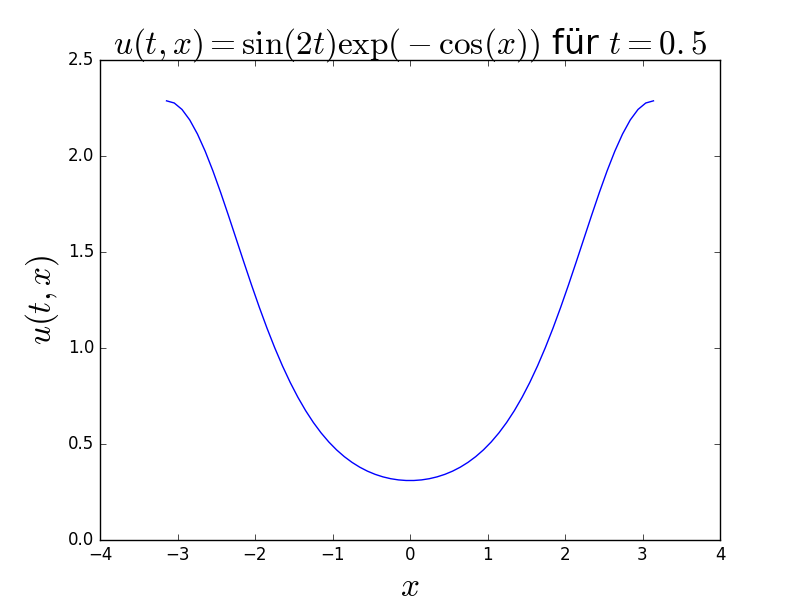
\includegraphics[width=\linewidth]{Figures/kgg_exact_solution_example1d.png}
  \caption{Exakte Lösung für $d=1$}
\endminipage
\minipage{0.5\textwidth}
  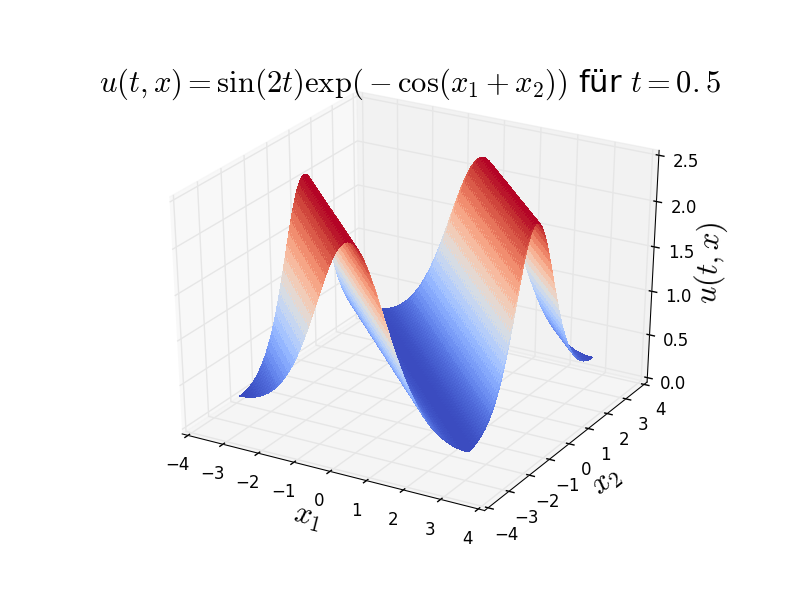
\includegraphics[width=\linewidth]{Figures/kgg_exact_solution_example2d.png}
  \caption{Exakte Lösung für $d=2$}
\endminipage
\captionsetup{labelformat=empty}
\caption{Lösung zum Zeitpunkt $t=0.5$ für die KGG (\ref{kgg}) mit Parametern $\alpha=1$, $
\beta(x)=4+d(\cos(\sum_{j=1}^dx_j)+\sin^2(\sum_{j=1}^dx_j))$.}
\end{figure}

Weitere --allerdings nicht-periodische-- Lösungen finden sich in \autocite{andreipolyanin2004}.

\section{Operator Splitting}
Um einen Ansatz für numerische Approximationen an die Lösung der KGG zu erhalten bietet sich ein klassischer Operator Splitting Ansatz an. Dabei wiederholen wir an dieser Stelle zuerst kurz die relevante Approximationstheorie und diskutieren mögliche Varianten.
\todo[inline]{Operator Splitting Theorie; Strang Splitting; Unsere Anwendung auf KGG; WaveSolver und LinhypSolver; Stabilität ohne CFL für $w=1$?}
\todo[inline]{Benötige Buch: Geometric Numerical Integration
Structure-Preserving Algorithms for Ordinary Differential Equations, Springer, Kap II.3 bis II.5}
\subsection{Generelle Idee}
Angenommen wir stehen vor dem Problem die Differentialgleichung 
\begin{equation}
\label{gencompdgl}
\dt{u}(t)=(A+B)u(t), \, t>0, \quad u(0)=u_0
\end{equation}
zu lösen. Dabei ist im einfachsten Fall $u$ eine vektorwertige Funktion und $A$ bzw. $B$ zwei Matrizen.\\
Sind aufgrund der Struktur der Matrizen --beispielsweise könnte $A$ eine obere und $B$ eine untere Dreiecksmatrix sein-- die Gleichungen 
\begin{align*}
\dt{v}(t)&=Av(t), \quad v(0)=v_0\\
\dt{w}(t)&=Bw(t), \quad w(0)=w_0
\end{align*}
deutlich einfacher zu lösen als die Gleichung (\ref{gencompdgl}), so lässt sich aus den Lösungen $v$ und $w$ dennoch eine Approximation an $u$ gewinnen.\\
Wir \emph{teilen} (engl. split) die Gleichung also in zwei neue Gleichungen auf. Häufig lässt sich dann eine der gewonnen Gleichungen sogar exakt lösen. Dieser Ansatz funktioniert auch für (nicht-lineare) Operatoren anstelle von Matrizen.\\
Diese zentrale Idee werden wir verwenden, um die KGG 
\begin{equation*}
\dtt{u}(t,x)=\alpha\Laplace u(t,x)-\beta(x)u(t,x)
\end{equation*}
zu splitten. Dabei wird der Operator $\alpha\Laplace$ in $A$ einfließen und $-\beta(x)$ in $B$. Man beachte jedoch, dass die zeitliche Ableitung zweiter Ordnung von $u$ eine Umschreibung in ein System erster Ordnung erfordert, bevor ein Splittingansatz sinnvoll ist.

\subsection{Lie-Trotter und Strang Splitting}
Wir beginnen mit einer rigerosen Einführung in Splitting Verfahren. Als zentrales Ergebnis werden wir dabei das Strang Splitting erhalten, welches einen Fehler $\mathcal{O}(\deltat^2)$ in Abhängigkeit von der Zeitschrittweite $\deltat$ besitzt.\\
Die folgende Einführung ist angelehnt an \autocite{patrickdiplom}, welche wiederum aus \autocite[Kapitel II.3 bis II.5]{HairerLubichWanner} übernommen wurde.
\begin{mathdef}[Fluss einer Differentialgleichung]
Der Fluss $\varphi_t$ einer reversiblen Differentialgleichung
\begin{equation}
\label{orddgl}
\partial_t \, y=f(y),\quad y(0)\:\text{ gegeben}
\end{equation}
mit $f\colon \R^d\to\R^d$ ist die injektive Abbildung, die einem gegebenen $y_0$ die exakte Lösung $y(t)$ zum Zeitpunkt $t$ zuordnet, wobei $y(0)=y_0$. Also gilt
\begin{equation*}
\varphi_t(y_0)=y(t)\enspace und\enspace y(0)=y_0
\end{equation*}
\end{mathdef}

Um Splitting Verfahren von möglichst höher Ordnung zu bekommen ist es wichtig, die einzelnen Teilverfahren bestmöglich zu kombinieren. Hierbei spielt das adjungierte Verfahren eine wichtige Rolle, da es dabei hilft, symmetrisierte Verfahren mit gerader Ordnung zu gewinnen.
\begin{mathdef}[Adjungiertes Verfahren]
Ist $\Phi_{\deltat}\colon\R^d\to\R^d$ ein Einschrittverfahren so definieren wir das adjungierte Verfahren $\Phi_{\deltat}^*$ als das Inverse des Einschrittverfahrens mit negativer Schrittweite $\deltat$, also \[\Phi_{\deltat}^*\coloneqq\Phi_{-\deltat}^{-1}\]
Das bedeutet, dass $y_1=\Phi_{\deltat}^*(y_0)$ implizit durch $\Phi_{-\deltat}(y_1)=y_0$ definiert wird.\\
Ist $\Phi_{\deltat}^*=\Phi_{\deltat}$ so nennen wir das Verfahren symmetrisch.
\end{mathdef}
Beispielsweise sind das explizite Euler Verfahren $\Phi_{\deltat}^E$ und das implizite Euler Verfahren $\Phi_{\deltat}^{IE}$ zueinander adjungiert: 
\[\Phi_{-\deltat}^E(y_1)=y_0\implies y_1+(-\deltat)f(y_1)=y_0\implies y_1=y_0+\deltat f(y_1)=\Phi_{\deltat}^{IE}(y_0)\] \\
Ohne Beweis sei bemerkt, dass $(\Phi_{\deltat}^*)^*=\Phi_{\deltat}$ und 
\begin{equation}
\label{adjlemma}
(\Phi_{\deltat}\circ \Psi_{\deltat})^*=\Psi_{\deltat}^* \circ \Phi_{\deltat}^*
\end{equation}

\begin{mathdef}[Konsistenzordnung]
Wir sagen, dass eine numerische Methode zum Lösen von (\ref{orddgl}) (konsistenz) von Ordnung $p$ ist, wenn der lokale Fehler \[\Phi_{\deltat}(y(t))=\varphi_{\deltat}(y(t))+\mathcal{O}(\deltat^{p+1})\] erfüllt (für $y(\cdot)$ hinreichend glatt).
\end{mathdef}
\begin{maththeorem}[Ordnung des adjungierten Verfahrens, vgl. 
{\autocite[Theorem II.3.2]{HairerLubichWanner}}]
\label{adjfloworder}
Sei $\varphi_t$ der exakte Fluss von (\ref{orddgl}) und sei $\Phi_{\deltat}$ ein Einschrittverfahren von Ordnung $p$ welches 
\[\Phi_{\deltat}(y_0)=\varphi_{\deltat}(y_0)+C(y_0)\deltat^{p+1}+\mathcal{O}(\deltat^{p+2})\]
erfüllt. Dann ist das adjungierte Verfahren $\Phi_{\deltat}^*$ ebenfalls von Ordnung $p$ und erfüllt
\[\Phi_{\deltat}^*(y_0)=\varphi_{\deltat}(y_0)+(-1)^{p}C(y_0)\deltat^{p+1}+\mathcal{O}(\deltat^{p+2})\]
Ist insbesondere $\Phi_{\deltat}$ symmetrisch, so ist wegen $C(y_0)=(-1)^pC(y_0)$ die Ordnung $p$ gerade.
\end{maththeorem}
Nun zerlegen wir die ursprüngliche Gleichung (\ref{orddgl}) in zwei Teile
\[\partial_t \, y=f(y)=A(y)+B(y) \]
Das Aufteilen ist hierbei nicht eindeutig! Eine Möglichkeit im zweidimensionalen wäre zum Beispiel: $A=\text{P}_{(1,0)^T}f,\,B=\text{P}_{(0,1)^T}f$, wobei $\text{P}_v$ die Projektion auf $\text{span}(v)$ darstellt. Häufig --ebenso wie in unserem Fall der KGG-- ist die natürliche Aufteilung der Summe die Methode der Wahl.\\
Sind nun $\varphi_{\deltat}^A$ und $\varphi_{\deltat}^B$ die exakten Flüsse der Systeme
\begin{align}
\partial_t \, y&=A(y)\quad \text{und} \label{splitsimple1}\\ 
\partial_t \, y&=B(y) \label{splitsimple2}
\end{align}
so gewinnen wir daraus ein Verfahren zur Lösung der ursprünglichen Gleichung.\\
Hierzu starten wir von einem gegebenen Anfangswert $y_0$ und lösen das System (\ref{splitsimple1}) um einen Zwischenwert $y_{\onehalf}$ zu erhalten. Verwenden wir diesen als neuen Startwert für das System (\ref{splitsimple2}), so erhalten wir einen daraus einen Wert $y_1$, welcher eine Approximation an die Lösung $\varphi_{\deltat}(y_0)$ des ursprünglichen Systems ist.\\[1cm]
\noindent\begin{minipage}{0.3\textwidth}
\begin{tikzpicture}
  \matrix (m) [matrix of math nodes,row sep=3em,column sep=4em,minimum width=2em]
  {
     \, & y_1 \\
     y_0 & y_{\onehalf} \\};
  \path[-stealth]
    (m-2-1.east|-m-2-2) edge node [below] {$\varphi_{\deltat}^A$} (m-2-2)
    (m-2-2) edge node [right] {$\varphi_{\deltat}^B$} (m-1-2)
    (m-2-1) edge [dashed] node [above left] {$\Phi_{\deltat}$} (m-1-2);
\end{tikzpicture}
\begin{tikzpicture}
  \matrix (m) [matrix of math nodes,row sep=3em,column sep=4em,minimum width=2em]
  {
     y_{\onehalf} & y_1 \\
     y_0 & \, \\};
  \path[-stealth]
    (m-1-1.east|-m-1-2) edge node [above] {$\varphi_{\deltat}^A$} (m-1-2)
    (m-2-1) edge node [left] {$\varphi_{\deltat}^B$} (m-1-1)
    (m-2-1) edge [dashed] node [below right] {$\Phi_{\deltat}^*$} (m-1-2);
\end{tikzpicture}
\end{minipage}%
\hfill%
\begin{minipage}{0.7\textwidth}
Die Reihenfolge $A\to B$ ist willkürlich und kann auch umgekehrt werden. Tatsächlich sind die resultierenden Verfahren zueinander adjungiert wegen (\ref{adjlemma}) und der Tatsache, dass der exakte Fluss wegen $y_1=\varphi_{-\deltat}^{-1}(y_0)=\varphi_{\deltat}^*(y_0)=\varphi_{\deltat}(y_0)$ als symmetrisches Einschrittverfahren auffassbar ist. Kurz:\\
$\Phi_{\deltat}=\varphi_{\deltat}^B \circ \varphi_{\deltat}^A$\\
$\Phi_{\deltat}^*=\varphi_{\deltat}^A \circ \varphi_{\deltat}^B$ 
\end{minipage}
\todo[inline]{how to get strang, visualize with tikz and why strang is order2, also fast strang}

\begin{maththeorem}[Ordnung des Lie-Trotter Splittings]
Das Lie-Trotter Splitting $\Phi_{\deltat}=\varphi_{\deltat}^B \circ \varphi_{\deltat}^A$ und sein adjungiertes $\Phi_{\deltat}^*=\varphi_{\deltat}^A \circ \varphi_{\deltat}^B$ sind von Ordnung $p=1$.
\end{maththeorem}
\begin{proof}
Die Taylorreihe von $\varphi_{\deltat}$ lässt sich darstellen als 
\[\varphi_{\deltat}(y_0)=y_0+\deltat f(y_0)+\frac{\deltat^2}{2}f^\prime(y_0)f(y_0)+\mathcal{O}(\deltat^3)\]
Diese vergleichen wir nun mit der Taylorreihe des Splittings
\begin{align*}
\left(\varphi_{\deltat}^B \circ \varphi_{\deltat}^A\right)(y_0)&=
\varphi_{\deltat}^B\left(y_0+\deltat f^A(y_0)+\frac{\deltat^2}{2}f^{\prime A}(y_0)f^A(y_0)+\mathcal{O}(\deltat^3)\right)\\
&=\left(y_0+\deltat f^A(y_0)+\frac{\deltat^2}{2}f^{\prime A}(y_0)f^A(y_0)\right)
+\deltat f^B\left(y_0+\deltat f^A(y_0)+\mathcal{O}(\deltat^2)\right)\\
&\quad+\frac{\deltat^2}{2}f^{\prime B}\left(y_0+\mathcal{O}(\deltat)\right)f^B\left(y_0+\mathcal{O}(\deltat)\right)+\mathcal{O}(\deltat^3)\\
&=y_0+\deltat f(y_0)+\frac{\deltat^2}{2}f^\prime(y_0)f(y_0)\\
&\quad+\frac{\deltat^2}{2}\left(f^{\prime B}(y_0)f^A(y_0)-f^{\prime A}(y_0)f^B(y_0)\right)+\mathcal{O}(\deltat^3)
\end{align*}
so bekommen wir den Fehler $\varphi_{\deltat}(y_0)-\left(\varphi_{\deltat}^B \circ \varphi_{\deltat}^A\right)(y_0)=\mathcal{O}(\deltat^2)$ und die Ordnung $p=1$. Mit Satz \ref{adjfloworder} ist das adjungierte Verfahren ebenfalls von Ordnung $p=1$.
\end{proof}
